
\documentclass[a4paper,landscape]{article}


\usepackage{tikz}
\usetikzlibrary{arrows}
\usetikzlibrary{fit,positioning, backgrounds}

\begin{document}

\begin{figure}
	\centering
	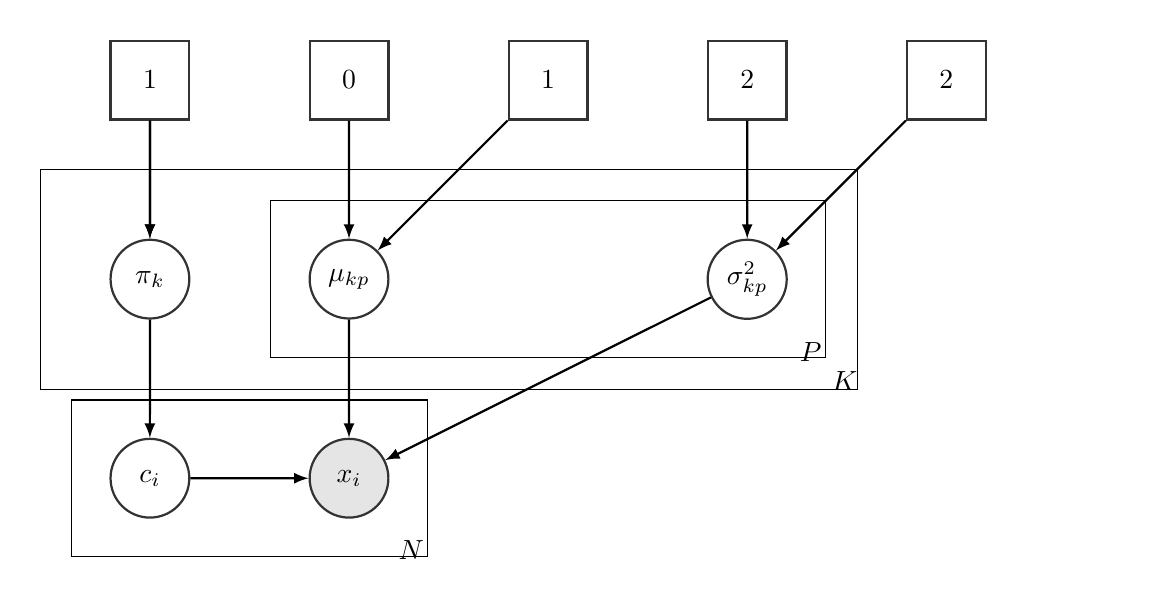
\begin{tikzpicture}[background rectangle/.style={fill=white!1}, show background rectangle, scale=.6, auto,>=latex']
		\tikzstyle{main}=[circle, minimum size = 10mm, thick, draw =black!80, node distance = 15mm]
		\tikzstyle{connect}=[-latex, thick]
		\tikzstyle{box}=[rectangle, draw=black!100]
		%\node[main] (k) {$K$ };
		\node[main, rectangle] (kappa) {$1$};
		\node[main, rectangle] (xi) [left =of kappa] {$0$ };
		\node[main, rectangle] (alpha) [left =of xi] {$1$ };
		\node[main, rectangle] (alpha2) [right =of kappa] {$2$ };
		\node[main, rectangle] (beta) [right =of alpha2] {$2$ };
		\node[main] (pi) [below =of alpha] {$\pi_k$ };
		\node[main] (c_i) [below =of pi] {$c_i$};
		\node[main] (mu) [below=of xi] {$\mu_{kp}$};		
		\node[main] (sigma) [below =of alpha2] {$\sigma^2_{kp}$};
		\node[main, fill = black!10] (x_i) [below =of mu] {$x_i$};
		\node[rectangle, inner sep=-0.5mm, fit= (c_i) (x_i),label=below right:$N$, xshift=13mm, yshift=-2mm] {};
		\node[rectangle, inner sep=4.8mm,draw=black!100, fit= (c_i) (x_i)] {};
		\node[rectangle, inner sep=-0.8mm, fit= (mu) (pi) (sigma),label=below right:$K$, xshift=43mm, yshift=-6mm] {};
		\node[rectangle, inner sep=8.8mm, draw=black! 100, fit= (mu) (pi) (sigma)] {};
		\node[rectangle, inner sep=-0.5mm, fit= (mu) (sigma),label=below right:$P$, xshift=26mm, yshift=-2mm] {};
		\node[rectangle, inner sep=4.8mm, draw=black! 100, fit= (mu) (sigma)] {};
		\path 
		%(k) edge [connect, bend right=30] (pi)
		%(k) edge [connect, bend left=10] (c_i)
		%(k) edge [connect, bend left=30] (mu)
		%(k) edge [connect] (sigma)
		(alpha) edge [connect] (pi)
		(pi) edge [connect] (c_i)
		(alpha) edge [connect] (pi)
		(c_i) edge [connect] (x_i)
		(mu) edge [connect] (x_i)
		(sigma) edge [connect] (x_i)
		(xi) edge [connect] (mu)
		(kappa) edge [connect] (mu)
		(alpha2) edge [connect] (sigma)
		(beta) edge [connect] (sigma)
		%(k) edge[connect, bend right=30] (x_i)
		;
	\end{tikzpicture}
	\caption{Directed acyclic graph for the Bayesian mixture of Gaussians used.}
	\label{fig:simpleMixNormals}

\end{figure}

\end{document}